\chapter{Testing and Analysis}
\label{ch:testing}
\chaptermark{Fith Chapter Heading}


\section{Testing}
The best test for my system is to use it in realistic scenario.


\begin{figure}[t]
    \centering
    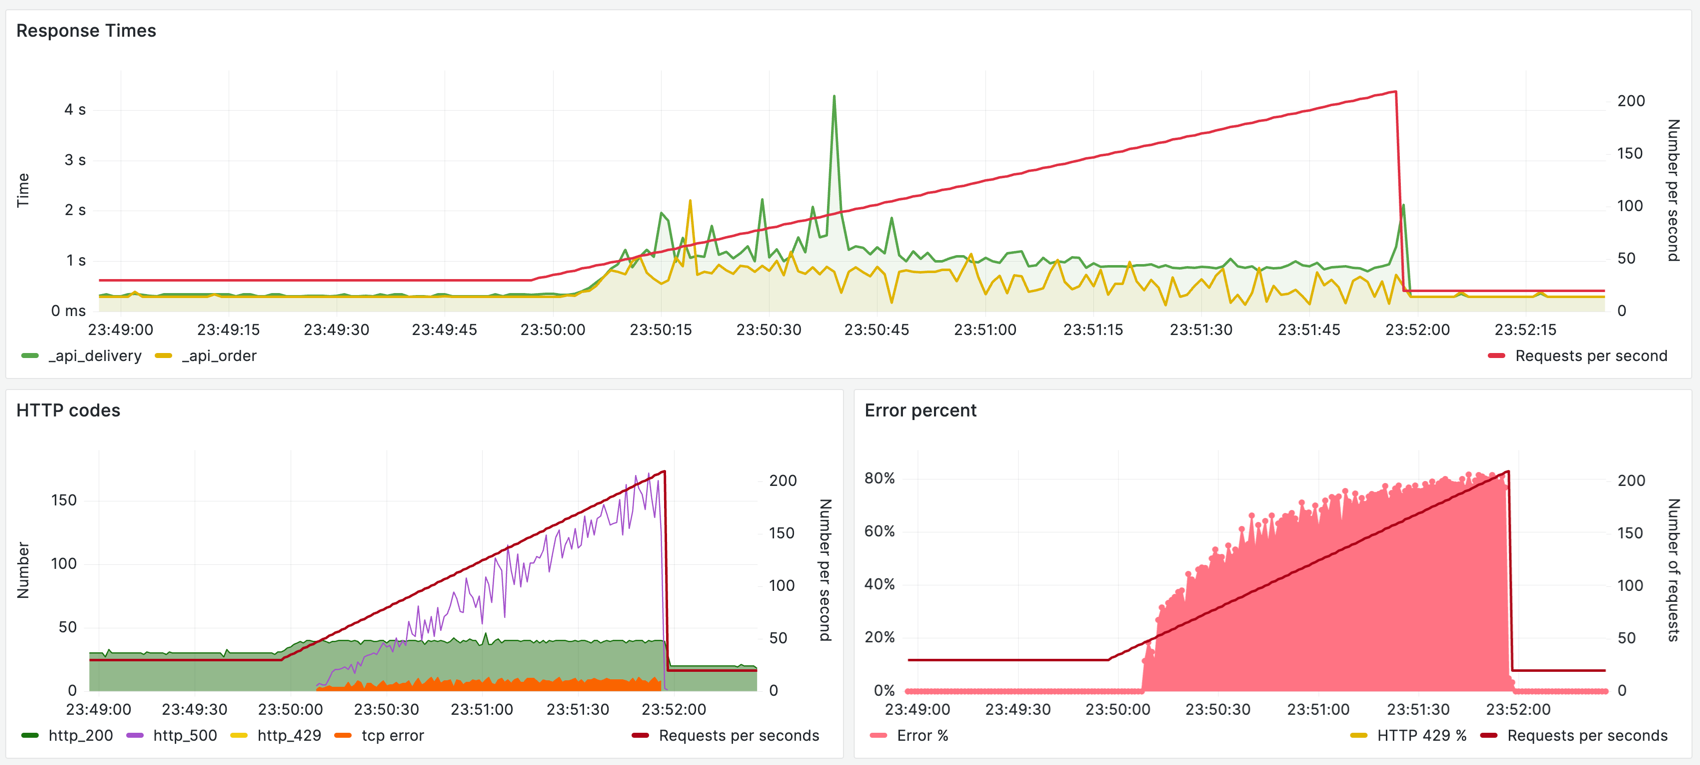
\includegraphics[height=\textheight,width=\textwidth,keepaspectratio]{cb_disabled.png}
    \caption{cb disabled}
    \label{fig:cb_disabled}
\end{figure}

\begin{figure}[t]
    \centering
    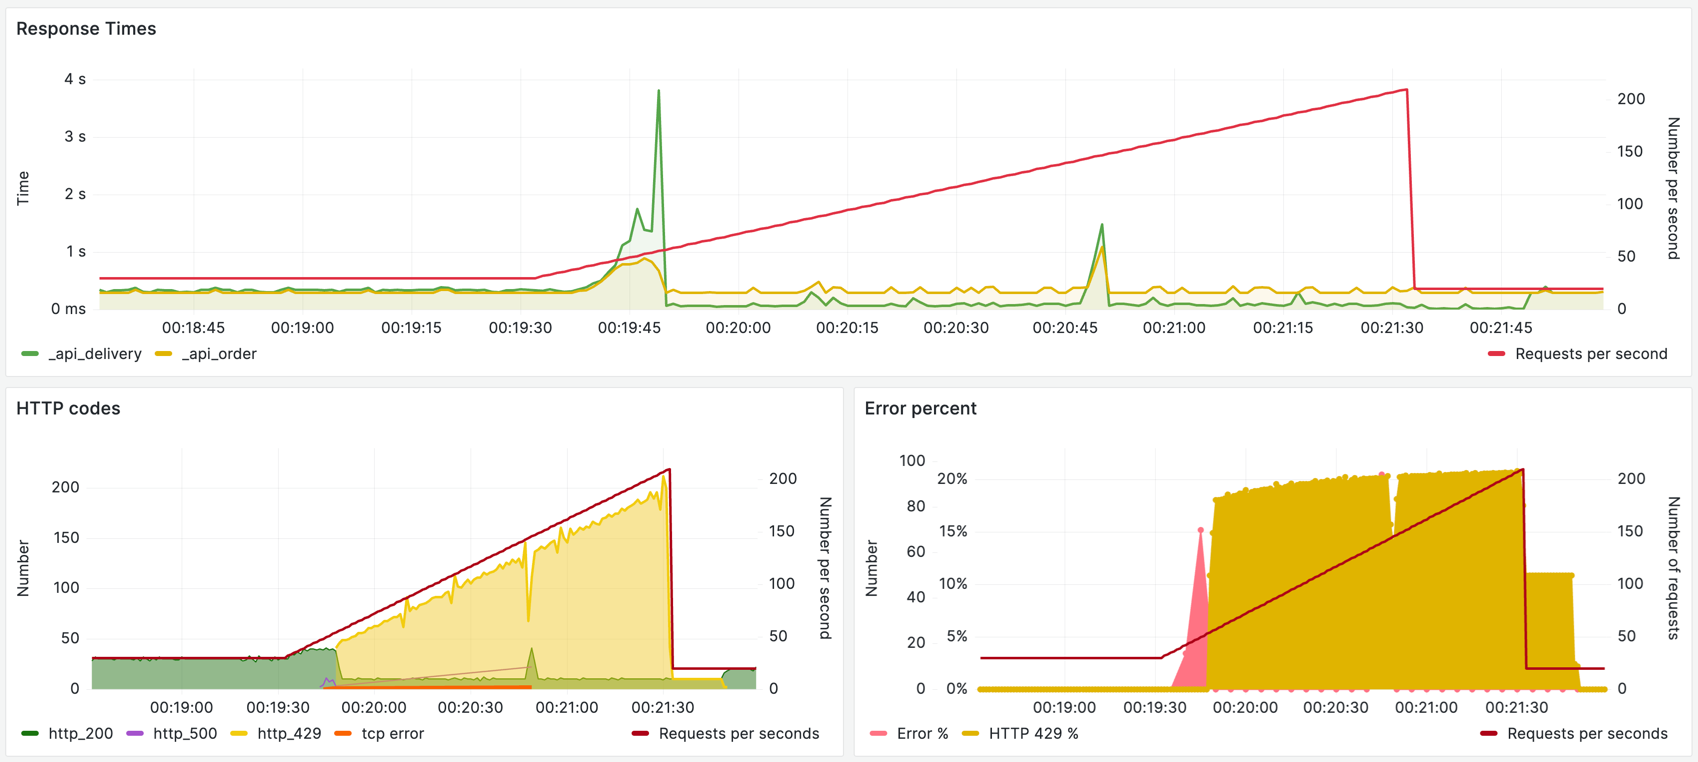
\includegraphics[height=\textheight,width=\textwidth,keepaspectratio]{cb_15.png}
    \caption{cb 15\%}
    \label{fig:cb_15\%}
\end{figure}

\begin{figure}[t]
    \centering
    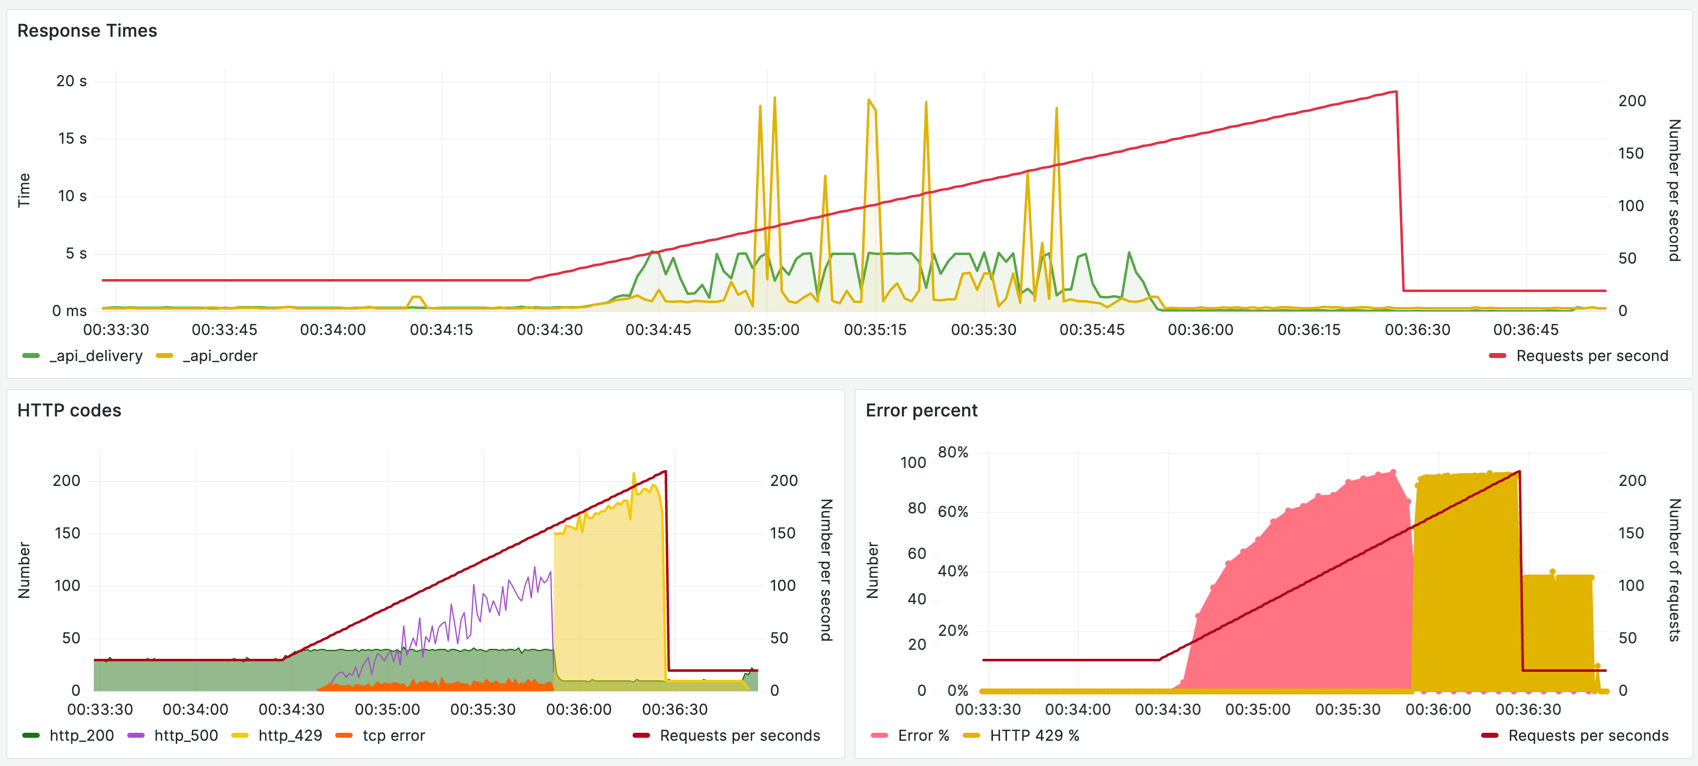
\includegraphics[height=\textheight,width=\textwidth,keepaspectratio]{cb_75.png}
    \caption{cb 75\%}
    \label{fig:cb_75\%}
\end{figure}

\subsection{Test system description}\label{subsec:test_system_description}

\subsection{Description of the test}\label{subsec:test_description}

\subsection{Execution}\label{subsec:test_description}

\section{Analysis}
Say smth about that it really helpful

\section{Limitations of the system}
The main limitation of the system lies in Yandex Tank API system. It supports to execute only one test simultaneously.